\section{Significance}

Significance, represents the confidence level at which we can assert that a detected event is
indeed a \tth event rather than a product of background noise or other processes. A robust measurement of significance
ensures that the observations are not mere statistical fluctuations.

\subsection{Poisson Distribution}

In particle physics, data collected from collision events are assumed to occur randomly and independently, thus
following the principles of a Poisson distribution. A Poisson distribution is a discrete probability distribution that
expresses the probability of a given number of events occurring in a fixed interval of time or space, given a fixed
average rate of these events.

An illustrative example might be the number of phone calls received by a call center within an hour, assuming a constant
average rate. If the call center typically receives an average of 10 calls per hour, and the calls are independent of
each other, the number of calls received in any given hour can be modeled by a Poisson distribution with a mean of
$\lambda = 10$. However, in real-world applications, the assumption of a constant rate might not always hold. For
example, the probability of receiving a call at 1pm may differ substantially from that at 1am, reflecting variations in
call patterns throughout the day. Such complexities necessitate a more nuanced approach in actual implementations, where
time-dependent variations in the rate of occurrence may need to be considered.

For a Poisson process, the average number of events in an interval is designated by the parameter
$\lambda$, which is
the rate parameter. The probability of observing $k$ events in an interval is given by the equation:

\begin{equation}
    P(k \text{ events in interval}) = \frac{\lambda^k e^{-\lambda}}{k!}\,,
\end{equation}

where $e$ is the base of the natural logarithm, and $k!$ is the factorial of $k$.

\autoref{fig:poisson} shows the Poisson distribution for various values of $\lambda$.

\begin{figure}[htb]
    \centering
    \includegraphics[width=0.8\textwidth]{figures/poisson.pdf}
    \caption[Poisson distribution for various values of $\lambda$]
    {Poisson distribution for various values of $\lambda$. For large $\lambda$, the Poisson distribution
        approaches a Gaussian distribution.}
    \label{fig:poisson}
\end{figure}

\subsection[Central Limit Theorem]{\gls{clt}}

\glsreset{clt}

The Poisson distribution and the Gaussian (or Normal) distribution are linked by the \gls{clt}, one of the
fundamental theorems in probability theory and statistics.

The \gls{clt} states that the sum of a large number of independent and identically distributed random
variables, each of which may be arbitrarily distributed, will approximately follow a Gaussian distribution, regardless
of the shape of the original distribution. This is true provided the mean and variance of the original distributions are
finite.

For a Poisson process, consider that each event occurs independently. So, we can imagine that our $\lambda$ (average
number of events in a given time period) is the sum of several smaller, independent rates. For instance, $\lambda$ could
be the result of $n$ independent processes each with a rate of $\frac{\lambda}{n}$. Thus, our Poisson process with rate
$\lambda$ can be viewed as the sum of $n$ Poisson processes each with a rate $\frac{\lambda}{n}$.

So, what happens when $n$ is large and $\frac{\lambda}{n}$ is small? Each individual Poisson process will rarely
contribute an event to the sum, but there are a lot of them ($n$ is large). This is precisely the sort of condition
under which the \gls{clt} operates. As such, we expect for large $\lambda$ that the Poisson distribution
will start to look more and more like a Gaussian distribution, as the Poisson distribution is the sum of many
independent and identically distributed random variables.

Mathematically, a random variable $X$ that is Poisson-distributed with mean $\lambda$ can be approximated by a Gaussian
distribution with mean $\lambda$ and variance $\lambda$, if $\lambda$ is large. This is usually taken to mean $\lambda >
    20$ or $30$ (see \autoref{fig:poisson}). Thus, for a Poisson distribution with large $\lambda$, it can be
approximated as

\begin{equation}
    X \sim N(\lambda, \sqrt{\lambda})\,.
\end{equation}

This allows us to use Gaussian statistics for large $\lambda$, which are mathematically more tractable. In the context
of particle physics, the number of events is often large, so the Poisson distribution can be approximated by a Gaussian
distribution, allowing us to use Gaussian statistics to analyze the data.

In our context, each collision event in the \tth could either be a signal (in our case, a \tth event) or part of the
background (any other process). The events are counted, and the count follows a Poisson distribution.

\subsection{Significance}

In the context of particle physics, and scientific experiments in general, significance plays a crucial role in
hypothesis testing. Hypothesis testing is a statistical method used to make inferences or draw conclusions about a
population based on a sample of data. The methodology of hypothesis testing involves the formulation of two competing
hypotheses, the null hypothesis (H0) and the alternative hypothesis (H1). The null hypothesis is a statement about the
population that will be accepted if the sample data do not provide sufficient evidence that it is false. On the other
hand, the alternative hypothesis is a claim about the population that will be accepted if the sample data provide
sufficient evidence that it is true. In our case specifically, the null hypothesis is that \tth process does not exist,
which we either accept or reject based on the amount of evidence provided by the data.

The process of hypothesis testing involves collecting data and calculating a test statistic which is then compared to a
critical value to decide whether to accept or reject the null hypothesis. This is where the $p$-value comes into
play. The $p$-value is a probability that provides a measure of the evidence against the null hypothesis provided by the
data. A smaller $p$-value provides stronger evidence against the null hypothesis. If the $p$-value is below a
predetermined significance level, typically 0.05 or 0.01, the null hypothesis is rejected in favor of the alternative
hypothesis. \autoref{fig:p-values} shows the relationship between the $p$-value and the significance level.

\begin{figure}[htb]
    \centering
    \includegraphics[width=\textwidth]{figures/p-values.pdf}
    \caption[The relationship between the $p$-value and the significance level.]
    {The relationship between the $p$-value and the significance level. Note that $p$-value is defined for the
        two-tailed test, while in our case we concerned with the case where we have more events than expected. However,
        this is not a problem, as the the significance level computed would underestimate the true significance level,
        meaning that in reality we would expect even better results.}
    \label{fig:p-values}
\end{figure}

In particle physics, the null hypothesis often refers to the background-only hypothesis, i.e., the hypothesis that only
known \gls{sm} processes are occurring. The alternative hypothesis, on the other hand, includes both the
background and a potential new signal.

This is where we connect hypothesis testing to Poisson statistics. We model the number of observed events as a random
variable that follows a Poisson distribution, with an expectation value equal to the sum of the expected number of
background events ($b$) and signal events ($s$). If the actual observed number of events is significantly larger than the
expected number of background events, then we have evidence against the null hypothesis.

The "significance" in particle physics refers to how many standard deviations an observed result is away from the
expectation under the null hypothesis. If our data gives a result that is very unlikely under the null hypothesis (say,
less than a 0.01 chance), we have strong evidence against the null hypothesis. The significance $Z$ is, in essence, the
number of standard deviations that the observed data is away from the expectation under the null hypothesis, with $Z = 1$
corresponding to a $p$-value of about 0.16 (or 16\%), and $Z = 2$ corresponding to a $p$-value of about 0.023 (or 2.3\%).

\begin{align}
    Z(p) & = \cdfinv(1 - p) & p(Z) & = 1 - \cdf(Z) = \int_{Z}^{\infty} \frac{1}{\sqrt{2\pi}} e^{-\frac{x^2}{2}} dx
\end{align}

\begin{table}[htb]
    \centering
    \begin{tabular}{|c|c|c|c|c|c|}
        \hline
        Significance   & 1     & 2    & 3    & 4                 & 5                 \\
        \hline
        \rule{0pt}{15pt}
        $p$-value (\%) & 15.87 & 2.28 & 0.13 & $3 \cdot 10^{-5}$ & $3 \cdot 10^{-7}$ \\
        \hline
    \end{tabular}
    \caption{Table of significances and corresponding p-values.}
    \label{tab:significance}
\end{table}

We illustrate this with an example. Suppose we only expect background processes to occur. In other words, during a
measurement period, we expect to observe $b$ background events. However, we observe $n=b+s$ events. This
could be due to statistical fluctuations, or it could be due to the presence of a new signal. Because events follow the
Poisson distribution, which can be approximated by a Gaussian for large $B$ and $S$, we can use the Normal distribution
$N(b, \sqrt{b})$ to model the number of observed events. The $Z$-score is then given by:

\begin{equation}
    Z = \frac{n-b}{\sqrt{b}} = \frac{s}{\sqrt{b}}
\end{equation}

We should note, however that due to the approximation of the Poisson distribution by the Gaussian distribution, the
number of background events $b$ must be large enough for the $Z$-score to be meaningful.

In practice, such approximation is often used in the early stages of a search due to its simplicity. For more accurate
results, a more complex statistical model is used that also accounts for different \glspl{np} - systematic
uncertainties (\autoref{ch:Evaluation}, \cite{pract-stat-lhc, statistical} for more details):

\begin{align}
    q_0  & = -2 \frac{L(\mu=0, \hat{\hat{\bm{\theta}}}(\mu=0))}{L(\hat{\mu}, \hat{\bm{\theta}})} \, \text{ where $\hat{\mu} > 0$} \\
    Z    & = \cdfinv(1 - p) = \sqrt{q_0}                                                                                          \\
    p(Z) & = 1 - \cdf(\sqrt{q_0})
\end{align}

where $L$ is the profile likelihood
function\footnote{\url{https://statisticalmethods.web.cern.ch/StatisticalMethods/statisticaltests}}, $\mu$ is the
parameter of interest\footnote{For our case specifically, $\mu$ refers to the signal strength, and so it is set to $0$
    as the null hypothesis assumes that there is no signal.}, $\bm{\theta}$ are the \glspl{np}, $\hat{\mu}$ and
$\hat{\bm{\theta}}$ are the \glspl{mle} of $\mu$ and $\bm{\theta}$ respectively, and $\hat{\hat{\bm{\theta}}}$ is the
\gls{mle} of $\bm{\theta}$ for a fixed value of $\mu$.

This provides a powerful tool for identifying new phenomena in particle physics. If the significance of a signal exceeds
a certain threshold (often $5\sigma$ in particle physics, corresponding to a $p$-value of about $3\cdot10^{-7}$), the
signal is considered a discovery.

For our experiments, we conduct the more precise calculation of significance once the best network is selected. However,
to get an estimate of what we can expect, we use the approximation described above to calculate the significance during
the model selection. It is important to note that when optimizing for significance, the \argmax strategy is usually not
optimal, so the threshold scanning (or working point optimization) is performed (see \autoref{fig:threshold-scan}):

\begin{figure}[htb]
    \centering
    \begin{subfigure}[t]{0.47\textwidth}
        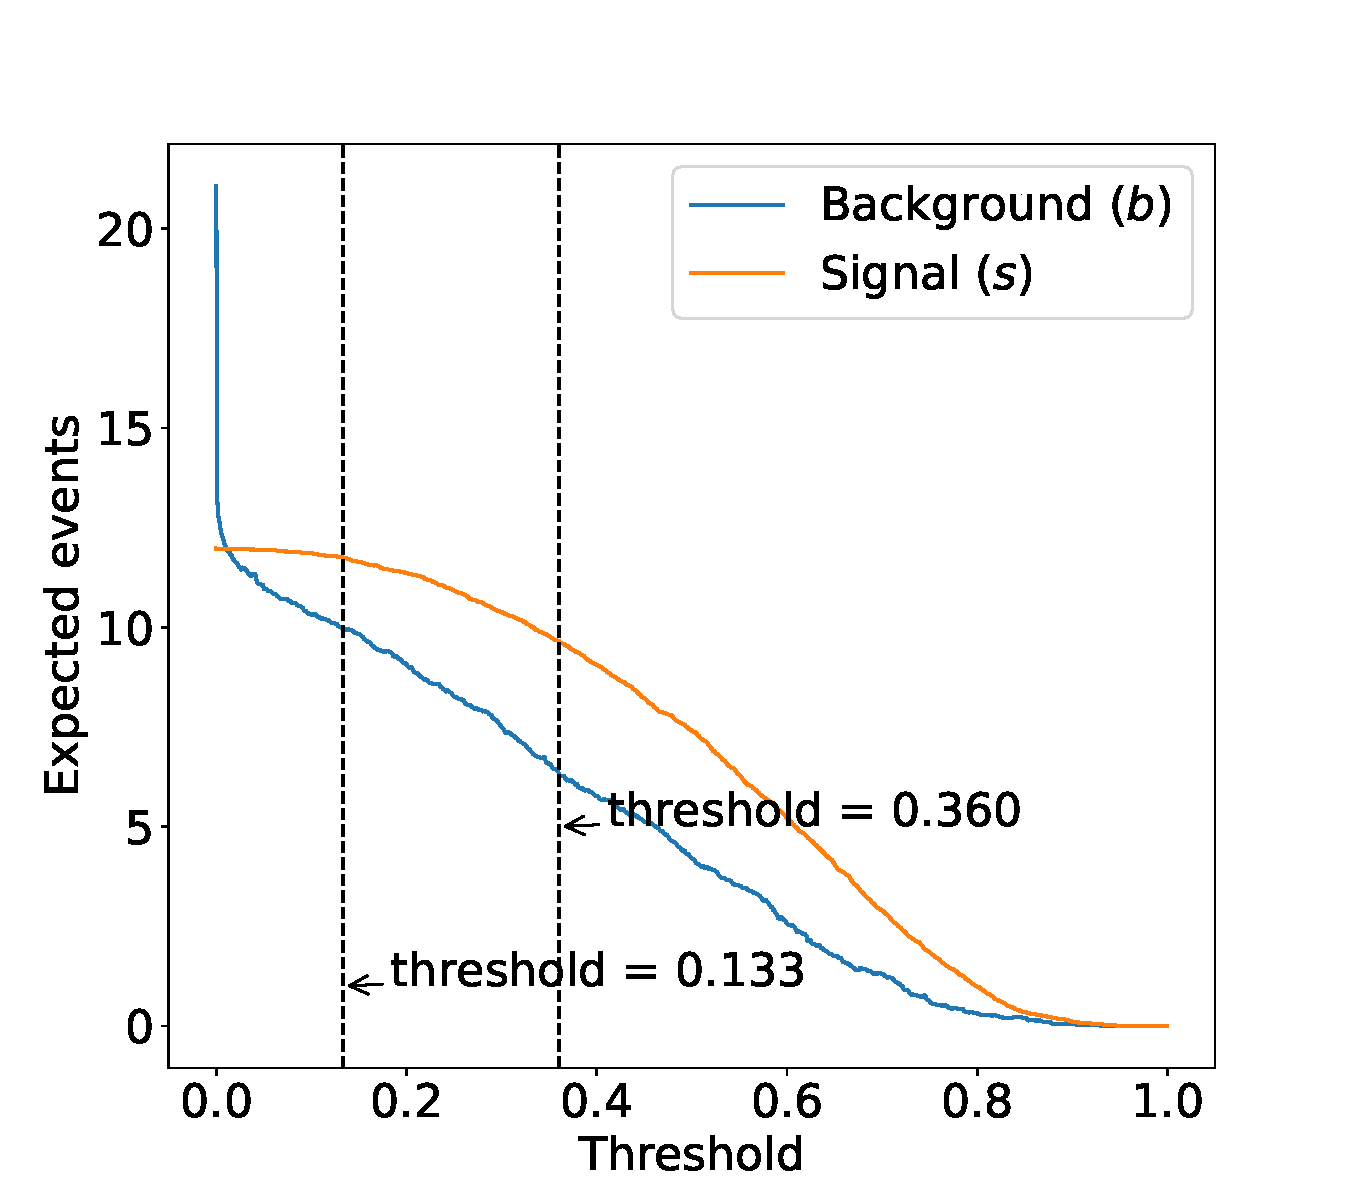
\includegraphics[width=\textwidth]{figures/ml/significance/yield.pdf}
        \caption[Influence of the threshold on the \tth and background processes' yields.]
        {Influence of the threshold on the \tth and background processes' yields. As the threshold increases,
            the number of true positives, as well as false positives, decreases.}
        \label{fig:signal-yield}
    \end{subfigure}
    \begin{subfigure}[t]{0.47\textwidth}
        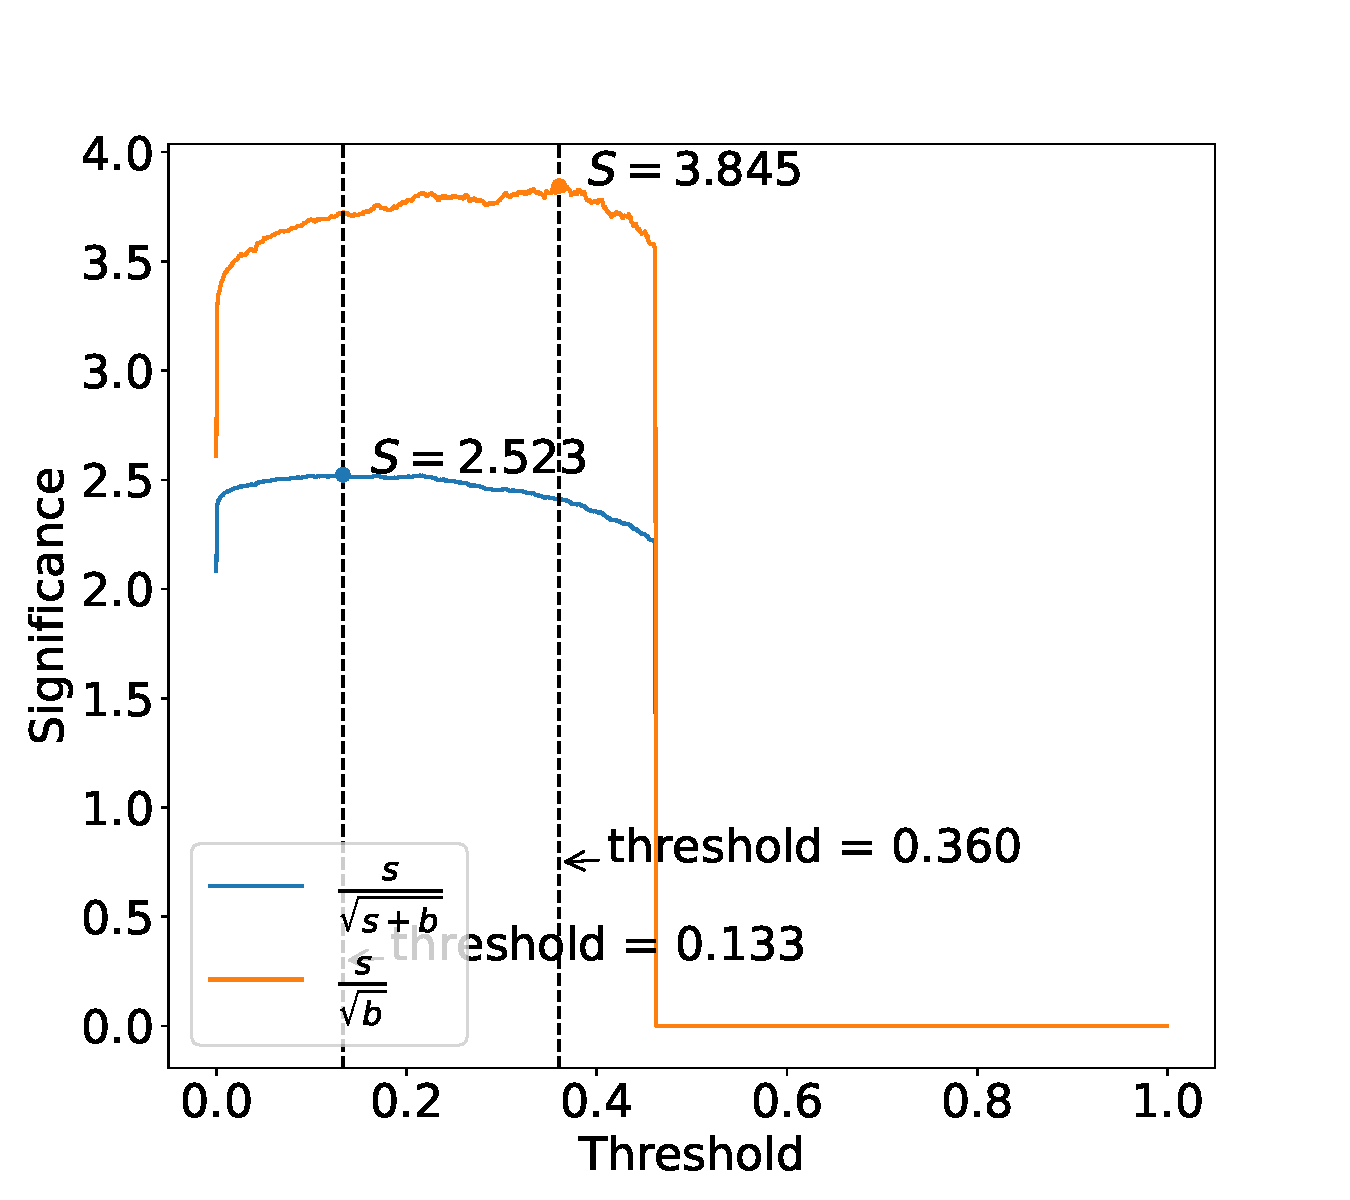
\includegraphics[width=\textwidth]{figures/ml/significance/thresholds.pdf}
        \caption[Influence of the threshold on the significance.]
        {Influence of the threshold on the significance. Two approximations are used. As the threshold changes, the
            significance changes accordingly. The threshold that maximizes the significance is chosen.}
        \label{fig:threshold-scan}
    \end{subfigure}
    \hfill
    \caption{Significance optimization.}
    \label{fig:significance-optimization}
\end{figure}

When we start with a threshold of 0, all events are essentially get classified as \tth, producing a high number of true
positives, but also a high number of false positives. As the threshold increases, the model gets more conservative and
starts classifying fewer events as \tth, reducing the number of true positives and false positives. For each threshold,
we compute both values for the significance and choose the threshold that maximizes the significance. As noted, this
is only an approximation, and the significance is calculated again using the better statistical model of significance.